\documentclass{article}
\usepackage{listings}
\usepackage{xcolor}
\usepackage{aligned-overset}
\usepackage{bookmark}
\usepackage{fancyhdr}
\usepackage{array}
\usepackage{appendix}
\usepackage{bm}
\usepackage{chapterbib}
\usepackage{float}
\usepackage[UTF8]{ctex}
\usepackage{geometry}
\usepackage{natbib}
\usepackage{url}
\usepackage{graphicx}
\renewcommand\arraystretch{2}
\usepackage{subfigure}
\usepackage{enumerate}
\geometry{left=2.18cm,right=2.08cm,top=1.84cm,bottom=1.84cm}
\usepackage{graphicx}
\pagestyle{plain}	
\usepackage{setspace}
\usepackage{indentfirst}
\usepackage{caption2}
\usepackage{datetime} %日期
\renewcommand{\today}{\number\year 年 \number\month 月 \number\day 日}
\renewcommand{\captionlabelfont}{\small}
\renewcommand{\captionfont}{\small}
\setlength{\parindent}{2em}
\lstset{language=Matlab}%代码语言使用的是matlab

\lstset{breaklines}%自动将长的代码行换行排版

\lstset{extendedchars=false}%解决代码跨页时,章节标题,页眉等汉字不显示的问题
\title{基于SIR模型对武汉新型冠状病毒疫情分析} 
\date{} 
\begin{document}
\begin{figure}
    \centering
    \includegraphics[width=8cm]{upc.png}
    \label{figupc}
\end{figure}
	\begin{center}
		\quad \\
		\heiti \fontsize{45}{17} \quad \quad \quad 
		\vskip 1cm
		\heiti \zihao{2} 《数学建模》中期大作业
	\end{center}
  \begin{center}
    \quad \\
    \quad \\
    \heiti \fontsize{45}{17} \quad \quad \quad 
    \vskip 1cm
    \heiti \zihao{3} 基于 SIR 模型对武汉新型冠状病毒疫情分析
    \vskip 2cm
  \end{center}

  \vskip 2cm
	\begin{quotation}
		\centering
    \begin{table}[H]
            \centering 
            \zihao{4}
            \begin{tabular}{|c|c|c|c|c|}
            
                \hline
                姓名& 张世琛 &李选  & 曹佳慧 & 张子锜 \\
                \hline
                学号&1804030401&1808010202& 1808010203&1808010201\\
                \hline
                班级&计科1802&计科1802& 计科1802&计科1802\\
                
                \hline
            \end{tabular}
        \end{table}
		\centering
		\vskip 4cm
		\today
	\end{quotation}

\thispagestyle{empty}
\newpage
\setcounter{page}{1}
\maketitle
\begin{abstract}
本文首先采用抽样检测法对2019-nCoV早期的模型的合理性及实用性进行了评价,然
后我们通过对传染病的共性及 2019-nCoV的特性的分析。得出三个基本假设并且把人群理
想化为三类 (S类 , I类 , R类 ),建立起基本的SIR模型,再对SIR模型中的三类人群间的相互转化关系的分析,由于 2019-nCoV的特性,可知 SIR模型中的两个参数 a(t), b(t)是以时间为变量的函数。我们根据武汉疫情的数据,通过多现实的数据拟合法分别得到 a(t), b(t)及 T结合,从而建立出模型。由于医疗条件的逐步改善,一定会制定出一套有效的治疗方案,甚至到后期的 2019-nCoV疫苗的研发。

本文利用数学软件(MATLAB)很好的实现了模型运算,并结合实际数据得出了人群与实
践的关系图。从图中可以很好的反映出各类人群的变化规律,他们的变化规律与实际变化相
吻合,从而证明了我们的模型基本符合要求。
\end{abstract}
%\section{引言}
          %\begin{figure}[h!]
          %      \centering
               % \includegraphics[width=12.5cm,height=5.5cm]{7.png}
           %     \caption{小木虫个人网站截图}
           %     \label{fig:universe}
           % \end{figure}
\section{问 题 重 述}
2019年底湖北省武汉市出现不明原因肺炎,于2020年初被世界卫生组织命名为新型冠状病毒,同期在全国范围内大面积爆发,对全国人民的日常生活造成巨大干扰,目前疫情在国内还未完全控制。基于此情况,我们认为有必要根据该病的特点,建
立合适的数学模型,分析合理的控制策略,预测疾病未来一段时间的发展趋势。
\section{问题的分析}
主要通过分析湖北(武汉)地区的受感染人数的变化规律,我们对该地区预测流行病的变
化趋势提出以下模型假设:
\begin{enumerate}
\item
将人群分为三类:
\begin{enumerate}
\item 易感染人数(疑似病例):用 S表示;
\item 病人数(已受感染者,即确诊者 ):用 I表示;
\item 移出者人数(包括“被治愈者”和“死亡者” ”,这部分人不再参与感染和被感染过程):用 R表示。

在SIR模型中以上三类人群之间存在两个转换的关系:
\newpage
\begin{figure}[h!]
                \centering
                \includegraphics[width=4.5cm,height=5cm]{11.png}
                \end{figure}
\end{enumerate}

\item 该地区人口不流动 (考虑到武汉已经封城,该假设是合理的 ),设最初易感染人数为 N
此时 I R均为 0.
\item 被隔离人群完全断绝与外界接触,不再具有传染性 (考虑到现有的医疗条件,该假设也
是合理的 )。
\end{enumerate}
\section{模型的分析与建立}
\subsection{初期数据的模拟}
传染病早期可以采用指数模型进行模拟
:$N ( t )=N_0 (1+k)^t$,当然,此情况是在社会来不
及防备以及群众不重视的基础上导致的。由于前期武汉市政府的不重视、人民对本次疫情的
忽视以及春节带来的附加作用,我们可以认为,新型冠状病毒前期是可以满足该指数模型的。
\begin{figure}[h!]
                \centering
                \includegraphics[width=4cm,height=10cm]{12.png}
                %\caption{武汉市人数统计表}
                \end{figure}
\begin{figure}[h!]
                \centering
                \includegraphics[width=12cm,height=8.7cm]{1.png}
                %\caption{武汉市人数统计图}
                \end{figure}
\begin{figure}[h!]
                \centering
                \includegraphics[width=15cm,height=8.5cm]{2.png}
                %\caption{武汉市人数统计图}
                \end{figure}
                1
\begin{figure}[h!]
由MATLAB 拟合出的人数曲线如上所示。武汉未在23日提供确诊人数,故将该点去
除后拟合。此外,MATLAB 给出的拟合结果如下:

增长模型:$f(x)=a(1+b)^x$

                \centering
                \includegraphics[width=3.5cm,height=3.5cm]{13.png}

   \leftline{显然,此模型只能适用于早期的预测。}
                %\caption{武汉市人数统计图}
                \end{figure}

\newpage

\section{模型的建立、求解}
建立SIR模型

易感染者,感染者,移出者之和是个恒量即$N=S+I+R$.假设病人康复后具有免疫力,
人与人之间有相同的接触率.最终由如下两种假设决定状态之间的转变率:
\begin{enumerate}
  \item 感染者的增长率是和感染者I与易感染者S的乘积成正比的
  \item 感染者I到移出者R的变化率是与感染者I成正比。
\end{enumerate}
基于以上两条得出模型的微分方程
 \begin{equation}
        \begin{split}
            \left\{
\begin{matrix}
\frac{dS}{dt}=-\alpha SI&\\ 
\frac{dI}{dt}=\alpha SI-\gamma I&\\ 
\frac{dR}{dt}=\gamma I&
\end{matrix}
\right.
        \end{split}
    \end{equation}
其中,$\alpha \quad \gamma$,𝑏都是以时间为变量的参数,$\alpha (t) $为日感染率,$\gamma (t)$为日移出率.
但是因为此疫情目前仍处于上升期,且相关数据较少,故按照以上微分方程组无法求出
$\alpha (t) $,$\gamma (t)$的解析解,因此我们先作数值计算。
参考多方资料后,我们设
$\alpha$=0.0000003,$\gamma$=0.0077266,I(0)=1,S(0)=1000000 (其
中感染率$\alpha$和移出率 $\gamma$都是根据官方所提供的数据估算出 ; 武汉市人口共有一千万,我们假设十分之一受到此次疫情的影响)

用MATLAB进行编程:
\begin{lstlisting}
function y = ill(t,x)
a=0.0000003;
b=0.0077266;
y=[a*x(1)*x(2)-b*x(1),-a*x(1)*x(2)]';
end

ts=[0:150];
x0=[1,1000000];
[t,x]=ode45('ill',ts,x0);
plot(t,x(:,1),t,x(:,2));
xlabel("天数")
ylabel("人数")
title("武汉省肺炎疫情人数预测图")
\end{lstlisting}

\begin{figure}[h!]
                \centering
                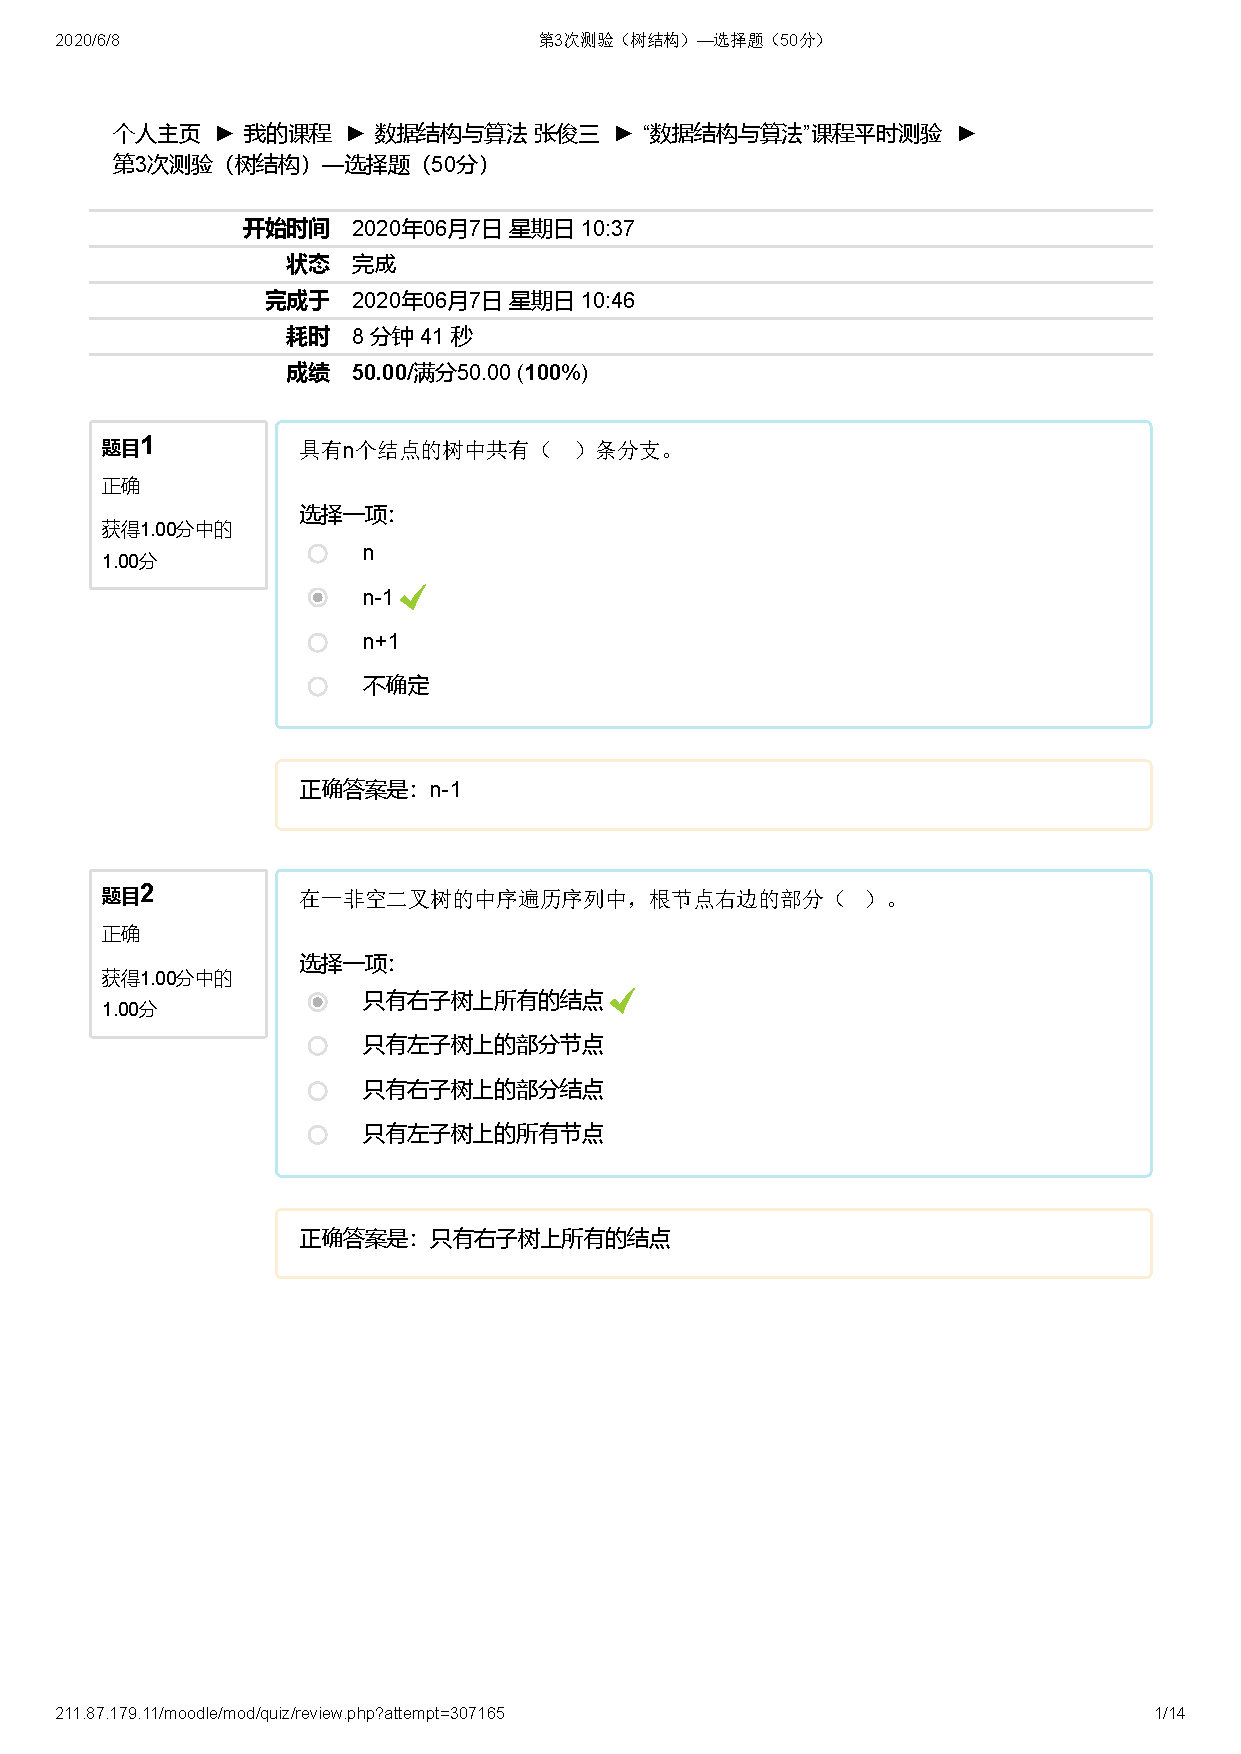
\includegraphics[width=15cm,height=8.5cm]{3.png}
                %\caption{武汉市人数统计图}
                \leftline{\quad \quad 上图是由
MATLAB求解微分方程后得出的结果。可以看到, 21天到 25天的数据,也
就是截止到 1月}
\leftline{26日24时,预测的数据都是符合实际情况的。}
                \end{figure}
\begin{figure}[H]
                \centering
                \includegraphics[width=18cm,height=5cm]{14.png}
                %\caption{武汉市人数统计图}
                \leftline{\quad \quad 但是,预测数据给出的结果显然是不符合实际情况的,随着疫情的扩张,感染率势必降
低,移出率势必提高。}
\leftline{因此,感染率$\alpha$和移出率$\gamma$不会是一个常数,该模型仍然有需要改进
的地方。}
                \end{figure}
\section{模型检验与分析}

\subsection{相轨线分析}
定义$\sigma =\frac{\alpha}{\gamma}$将原微分方程组化简:
$$\frac{dI}{dS}=\frac{1}{\sigma S}-1,I_{S=S_{0}}=I_{0}$$
容易求出此微分方程的解为:
$$I=(S_{0}+I_{0})-S+\frac{1}{\sigma} ln{\frac{S}{S_0}} $$
显然当
$S=\frac{1}{\sigma}$时I最大。对于基本模型来说,其$\frac{1}{\sigma}=\frac{0.0077266}{0.0000003}=25755$
\begin{figure}[h!]
                \centering
                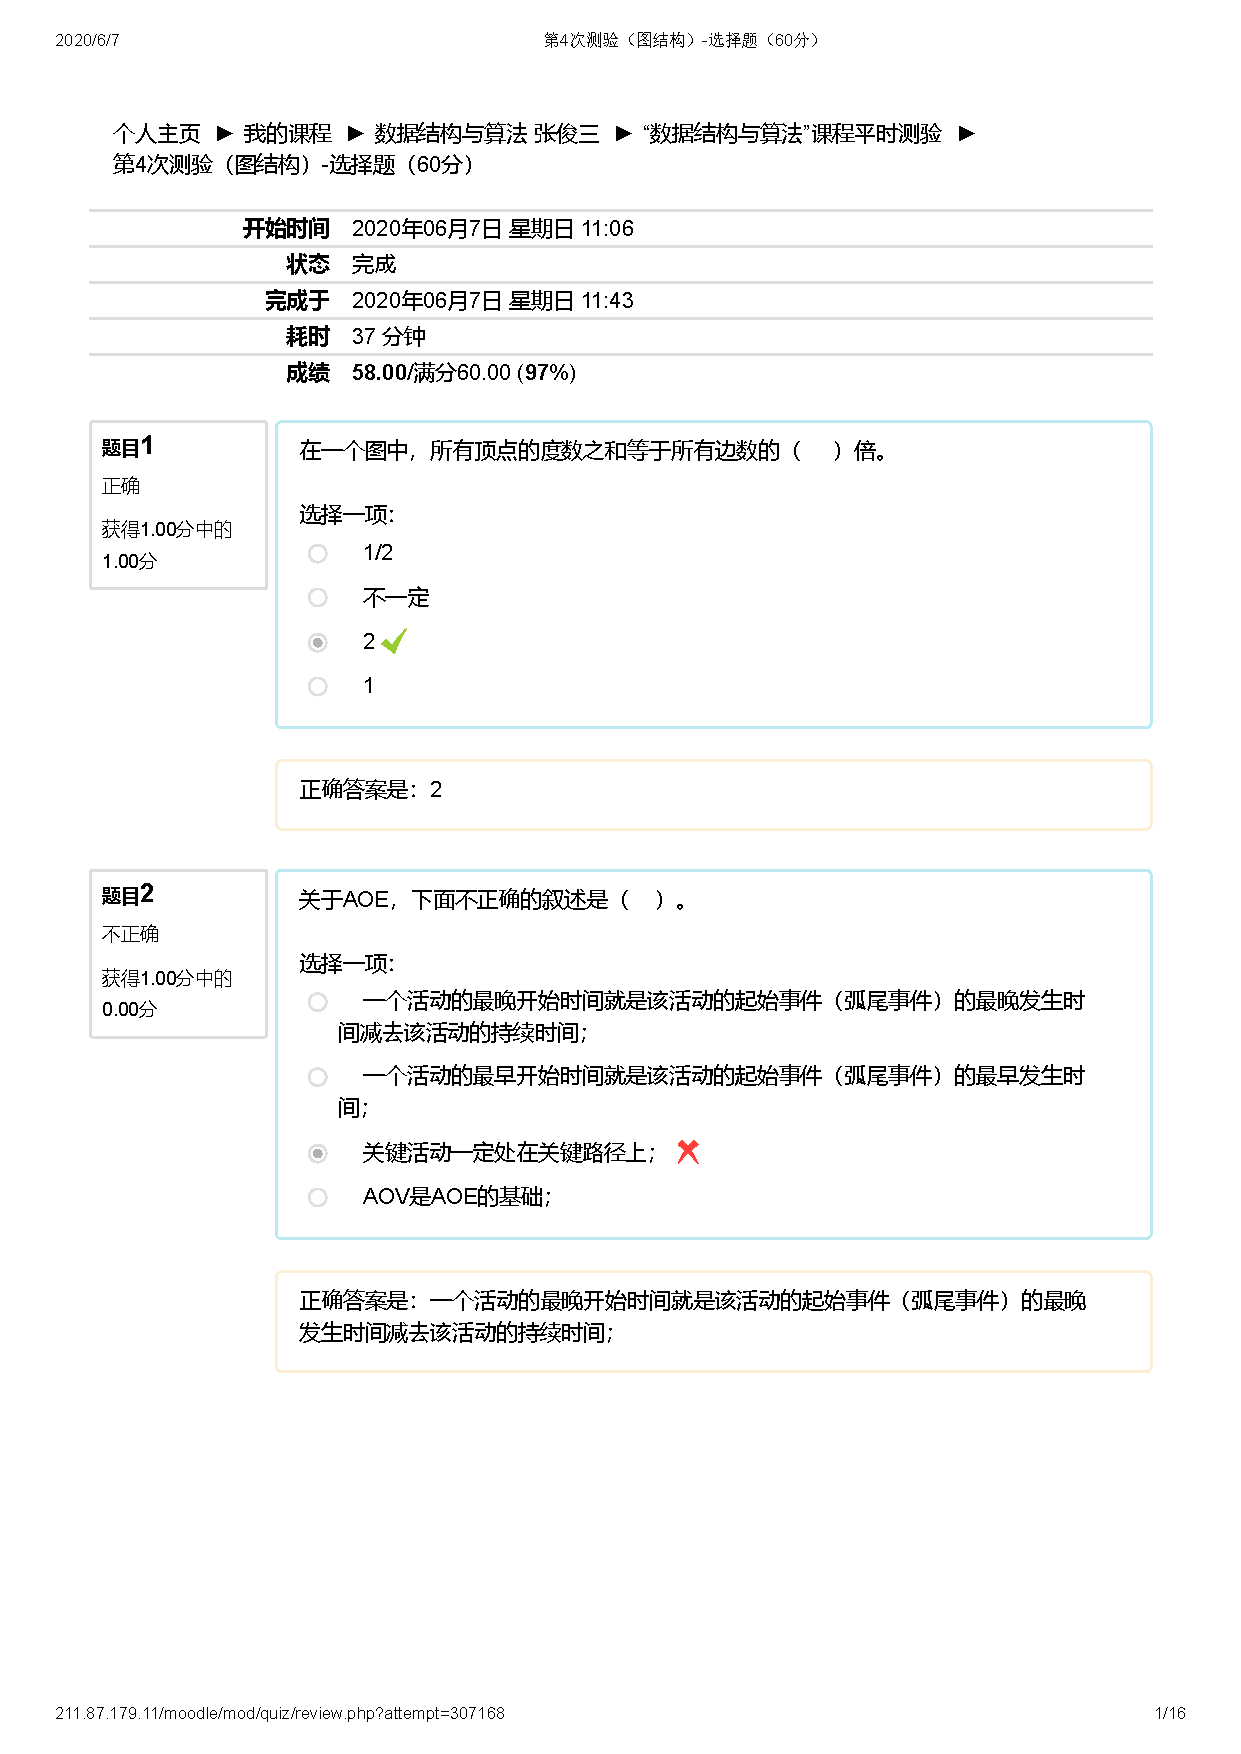
\includegraphics[width=15cm,height=8.5cm]{4.png}
                %\caption{武汉市人数统计图}
                \leftline{

              \quad \quad 由相图可知,
,1/𝜎所代表的是一个阈值, 当$S>frac{1}{\sigma}$时,传染病在蔓延 ; 当 $S<frac{1}{\sigma}$时,
传染病则不会蔓延。
              }
                \end{figure}
\subsection{模型的改进}
由前面分析可知,此模型对于前期疫情的预测比较准确,但是对于后期疫情的发展则显
然不符合实际结果。其原因是因为 感染率 $\alpha$和移出率 $\gamma$不会是一个常数。
后期传染率应呈
指数型下降。并将移出率用 sigmoid函数进行优化。
\begin{enumerate}
  \item 首先 保持移出率不变 ,优化感染率函数
  $$\alpha =0.0000003∗((stepfun(t,0)-stepfun(t,25))+stepfun(t,25)*
  e^{-0.02*(t-25)})$$
  \begin{figure}[h!]
                \centering
                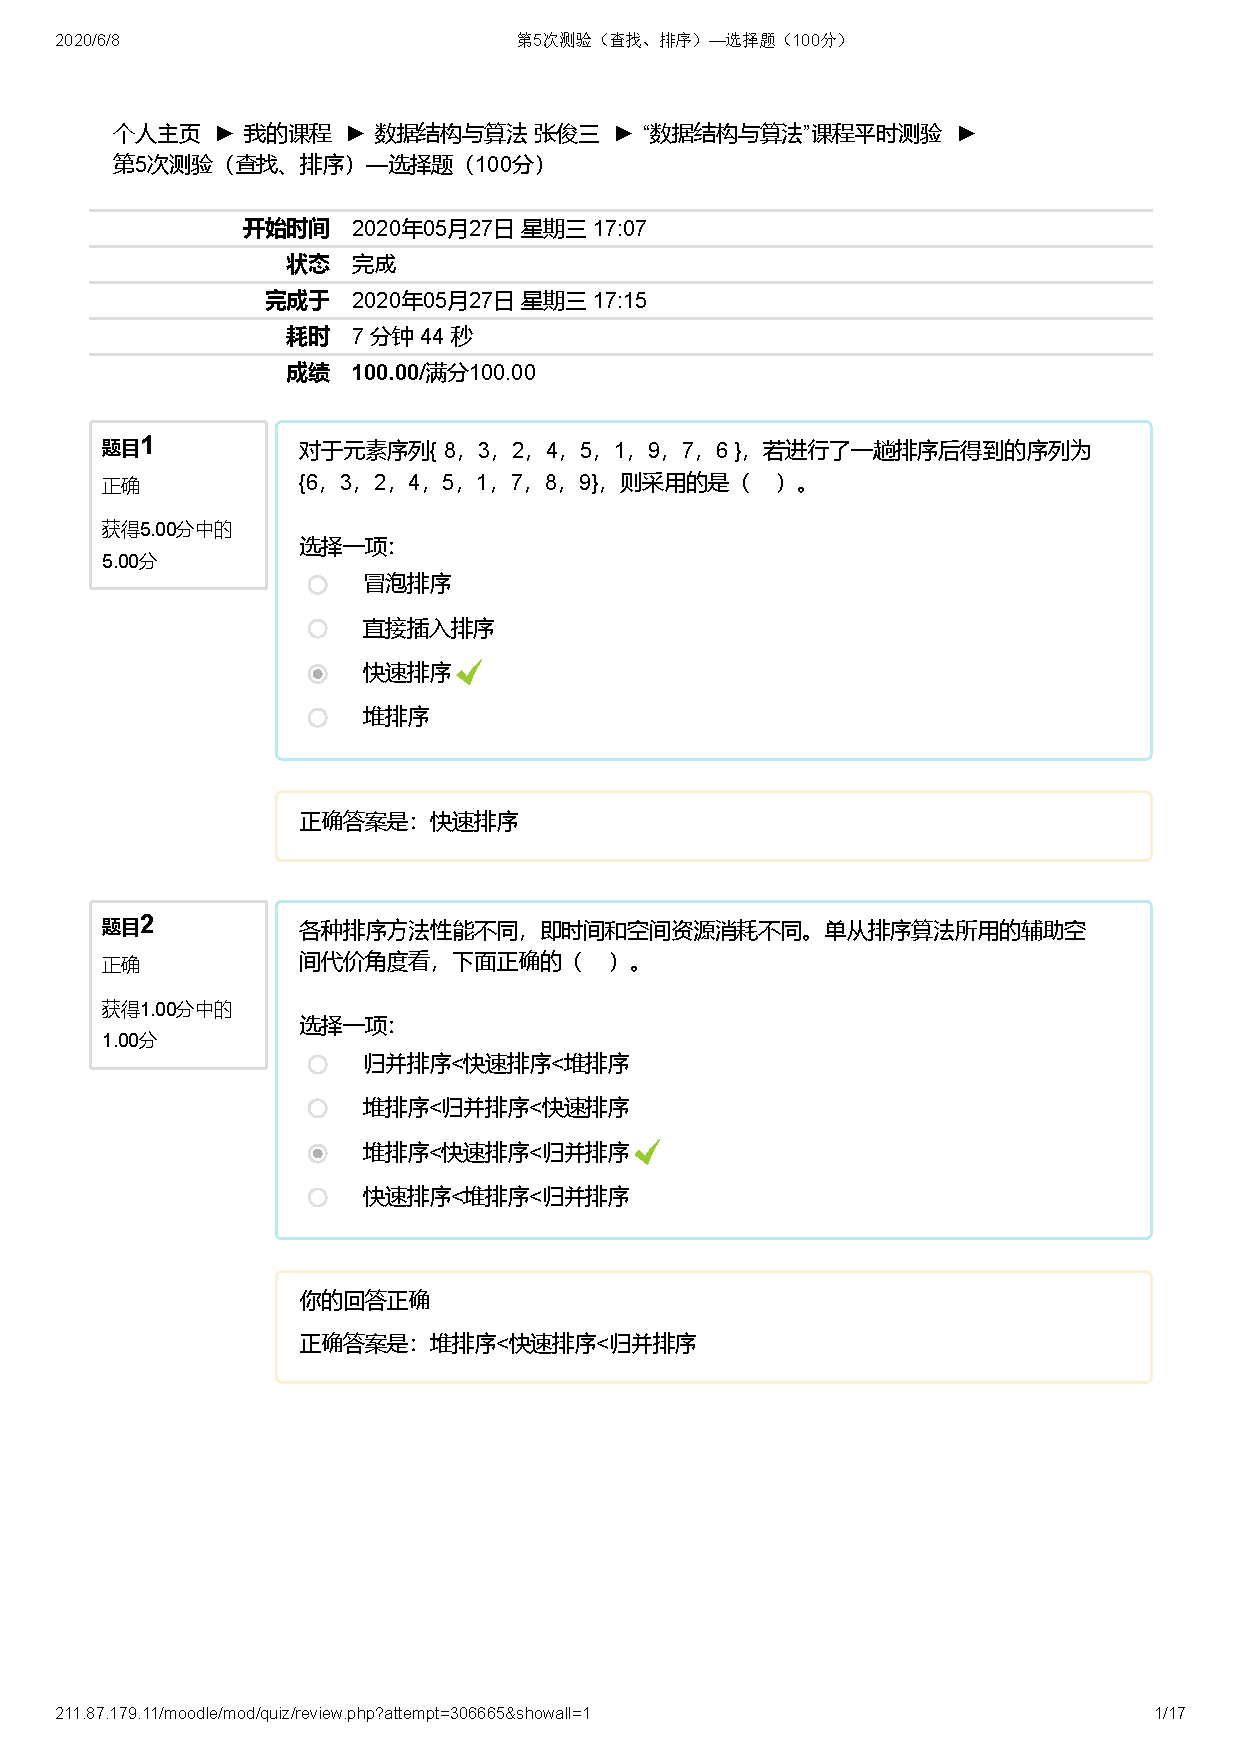
\includegraphics[width=15cm,height=7.8cm]{5.png}
              \leftline{\quad \quad 感染率曲线(第25 天时武汉市采取响应措施,故从该日起感染率下降)
由改进后的模型建立的预测图,}
\leftline{前期预测仍然符合预期,且大大缓解了高峰时期患病的人数。}
                \end{figure}
    \begin{figure}[h!]
                \centering
                \includegraphics[width=15cm,height=8.5cm]{6.png}
              \leftline{\quad \quad 下面改变感染率函数下降的斜率,由MATLAB 拟合出结果:}
                \end{figure}            
      \begin{figure}[h!]
                \centering
                \includegraphics[width=15cm,height=8.5cm]{8.png}
              \leftline{\quad \quad 增大感染率下降的梯度,可以有效的降低感染人数。}
                \end{figure}  
\item 在(1)的基础上改进移出率函数
$$\alpha = 0.0000003*((stepfun(t,0)-stepfun(t,25))+stepfun(t,25)*
e^{-0.05 ∗ (t-25)})$$
$$\gamma = 0.0077266*(stepfun(t, 0) +stepfun(t, 25)*(\frac{5}{1 + 
e^{-(t-28)}})$$  \\
\\
 \begin{figure}[h!]
                \centering
                \includegraphics[width=15cm,height=8.5cm]{7.png}
              \leftline{\quad \quad 在改进模型的情况下,我们发现,相比于(1)的结果,肺炎疫情在60 天左右即得到了有
效的控制,}
\leftline{且感染人数呈数十倍的下降。当然,预测的数据仍然具有一定的问题.}
                \end{figure}  
\item 灵敏度分析
\begin{enumerate}
\item 对$\alpha$做灵敏度分析
$$\alpha_1 = 0.0000003*((stepfun(t,0)-stepfun(t,25))+stepfun(t,25)*
e^{-0.05 ∗ (t-25)})$$
$$\gamma_1 = 0.0077266*(stepfun(t, 0) +stepfun(t, 25)*(\frac{5}{1 + 
e^{-(t-28)}})$$  
$$\alpha_2 = 0.0000003*((stepfun(t,0)-stepfun(t,25))+stepfun(t,25)*
e^{-0.045 ∗ (t-25)})$$ 
$$\gamma_2 = 0.0077266*(stepfun(t, 0) +stepfun(t, 25)*(\frac{5}{1 + 
e^{-(t-28)}})$$  
$$\alpha_3 = 0.0000003*((stepfun(t,0)-stepfun(t,25))+stepfun(t,25)*
e^{-0.055 ∗ (t-25)})$$
$$\gamma_3 = 0.0077266*(stepfun(t, 0) +stepfun(t, 25)*(\frac{5}{1 + 
e^{-(t-28)}})$$  
 \begin{figure}[h!]
                \centering
                \includegraphics[width=15cm,height=7cm]{9.png}
              \leftline{\quad \quad 如图可见,感染人数对
a的变化还是比较灵敏的。这对于现实中的疫情防控具有很好的
指导作用,}
\leftline{尤其是控后,如何快速的降低 感染率以便快速的控制疫情是防止疫情蔓延的重点。}
                \end{figure} 
                \newpage
\item 对$\gamma$做灵敏度分析
$$\alpha_1 = 0.0000003*((stepfun(t,0)-stepfun(t,25))+stepfun(t,25)*
e^{-0.05 ∗ (t-25)})$$
$$\gamma_1 = 0.0077266*(stepfun(t, 0) +stepfun(t, 25)*(\frac{5}{1 + 
e^{-(t-28)}})$$  
$$\alpha_2 = 0.0000003*((stepfun(t,0)-stepfun(t,25))+stepfun(t,25)*
e^{-0.05 ∗ (t-25)})$$ 
$$\gamma_2 = 0.0077266*(stepfun(t, 0) +stepfun(t, 25)*(\frac{4.5}{1 + 
e^{-(t-28)}})$$  
$$\alpha_3 = 0.0000003*((stepfun(t,0)-stepfun(t,25))+stepfun(t,25)*
e^{-0.05 ∗ (t-25)})$$
$$\gamma_3 = 0.0077266*(stepfun(t, 0) +stepfun(t, 25)*(\frac{5.5}{1 + 
e^{-(t-28)}})$$  
 \begin{figure}[h!]
                \centering
                \includegraphics[width=15cm,height=7cm]{10.png}
              \leftline{\quad \quad 同样,如何提高移出率
(主要是指治愈率 )也是疫情防控后的重点。}
                \end{figure} 
\end{enumerate}
\end{enumerate}           

\subsection{模型分析}
虽然改进后的模型能够对疫情做出比较理想的趋势分析,但是对于疫情后期的处理仍然
与真实情况有所偏差。主要是由 三 个原因导致的,
\begin{enumerate}
  \item SIR模型过于精简,将真实情况过度
理想化。本次疫情的感染不光是由感染者传染的,对于一部分易感人群,只要携带病原体,
均可以作为传染源,但是该部分人群在模型的建立当中并没有体现出来。
\item 本次疫情仍处
于上升期,且真实数据不足,加上湖北省政府前期的怠慢导致的数据异常,我们没有办法对
控前做一个很好的拟合,同样,对控后亦无从而知。 
\item 武汉市人口基数众多 ,且正逢春节
按照 官方的说法 ,在武汉封 城之前 ,有约 500万人离开武汉 。 这对于模型的 建立是一个极大
的挑战 ,因为 一般的模型都要求人口固定且无人口交流 。
\end{enumerate}
\section{参考文献}
\begin{enumerate}
\item 姜启源 谢金星 叶俊,《数学模型》(第三版),北京;高等教育出版社
\item 基于SIR模型和基本再生数的浙江省新型冠状病毒肺炎防控效果分析[J]. 李承倬,武文韬,潘振宇,邓玉皎,李筱,代志军,吕军.浙江医学.
\item 传染病传播模型综述[J]. 张发,李璐,宣慧玉.系统工程理论与实践. 
\item SARS流行病的SEIR动力学模型及其参数辨识[J]. 徐恭贤,冯恩民,王宗涛,谭欣欣,修志龙.黑龙江大学自然科学学报. 2005(04)
\item 传染病传播模型研究[J]. 余雷,薛惠锋,李刚.计算机仿真. 2007(04)
\end{enumerate}

\section{工作分工情况}
\begin{quotation}
    \centering
    \begin{table}[H]
            \centering 
            \zihao{4}
            \begin{tabular}{|p{4cm}<{\centering}|p{4cm}<{\centering}|p{4cm}<{\centering}|}
            
                \hline
                姓名& 分工 &打分 \\
                \hline
                张世琛&编程+写作&9.9\\
                \hline
                李选&建模&9.9\\
                \hline
                曹佳慧&写作+搜集数据&9.9\\
                \hline
                张子锜&写作+搜集数据&9.9\\
                \hline
            \end{tabular}
        \end{table}
  \end{quotation}

\end{document}